\begin{frame}{Complication for saddle point problems}
  \begin{columns}
    \begin{column}{0.2\textwidth}
      \[ \begin{pmatrix}
        A & B^T \\ B & 0
      \end{pmatrix} \]
    \end{column}
    \begin{column}{0.8\textwidth}
      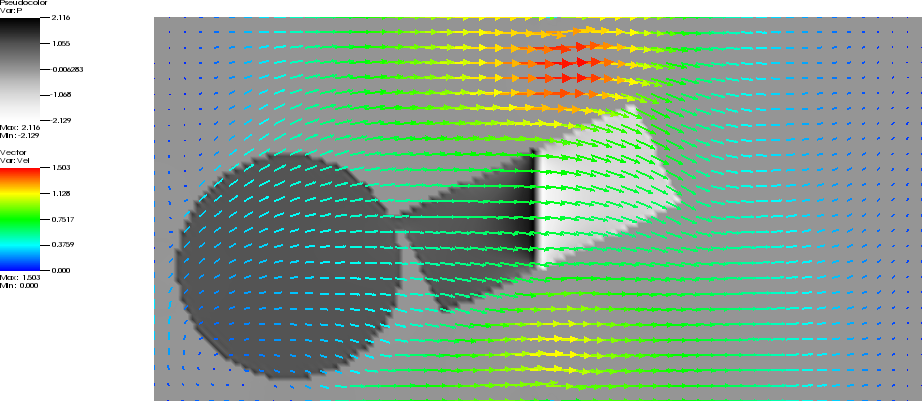
\includegraphics[width=\textwidth]{figures/MG/StokesDualProblem}
    \end{column}
  \end{columns}
  \begin{itemize}
  \item want uniform stability for coarse problem
    \begin{itemize}
    \item respect inf-sup condition, similar to fine grid
    \item make coarse grid mimic fine grid ($Q_2-P_1^{\text{disc}}$)
    \end{itemize}
  \item \emph{exact} representation of volumetric mode
    \begin{itemize}
    \item we can't cheat on conservation while upscaling
    \item naturally involves face integrals (inconvenient for recursive application)
    \item obtain similar quantity through solution of inhomogeneous Stokes problems
    \end{itemize}
  \item heuristic algebraic coarsening also possible [Adams 2004]
  \end{itemize}
\end{frame}
